\chapter{Diseño e implementación} % Main chapter title

\label{Chapter3} % Change X to a consecutive number; for referencing this chapter elsewhere, use \ref{ChapterX}

\definecolor{mygreen}{rgb}{0,0.6,0}
\definecolor{mygray}{rgb}{0.5,0.5,0.5}
\definecolor{mymauve}{rgb}{0.58,0,0.82}

%%%%%%%%%%%%%%%%%%%%%%%%%%%%%%%%%%%%%%%%%%%%%%%%%%%%%%%%%%%%%%%%%%%%%%%%%%%%%
% parámetros para configurar el formato del código en los entornos lstlisting
%%%%%%%%%%%%%%%%%%%%%%%%%%%%%%%%%%%%%%%%%%%%%%%%%%%%%%%%%%%%%%%%%%%%%%%%%%%%%
\lstset{ %
  backgroundcolor=\color{white},   % choose the background color; you must add \usepackage{color} or \usepackage{xcolor}
  basicstyle=\footnotesize,        % the size of the fonts that are used for the code
  breakatwhitespace=false,         % sets if automatic breaks should only happen at whitespace
  breaklines=true,                 % sets automatic line breaking
  captionpos=b,                    % sets the caption-position to bottom
  commentstyle=\color{mygreen},    % comment style
  deletekeywords={...},            % if you want to delete keywords from the given language
  %escapeinside={\%*}{*)},          % if you want to add LaTeX within your code
  %extendedchars=true,              % lets you use non-ASCII characters; for 8-bits encodings only, does not work with UTF-8
  %frame=single,	                % adds a frame around the code
  keepspaces=true,                 % keeps spaces in text, useful for keeping indentation of code (possibly needs columns=flexible)
  keywordstyle=\color{blue},       % keyword style
  language=[ANSI]C,                % the language of the code
  %otherkeywords={*,...},           % if you want to add more keywords to the set
  numbers=left,                    % where to put the line-numbers; possible values are (none, left, right)
  numbersep=5pt,                   % how far the line-numbers are from the code
  numberstyle=\tiny\color{mygray}, % the style that is used for the line-numbers
  rulecolor=\color{black},         % if not set, the frame-color may be changed on line-breaks within not-black text (e.g. comments (green here))
  showspaces=false,                % show spaces everywhere adding particular underscores; it overrides 'showstringspaces'
  showstringspaces=false,          % underline spaces within strings only
  showtabs=false,                  % show tabs within strings adding particular underscores
  stepnumber=1,                    % the step between two line-numbers. If it's 1, each line will be numbered
  stringstyle=\color{mymauve},     % string literal style
  tabsize=2,	                   % sets default tabsize to 2 spaces
  title=\lstname,                  % show the filename of files included with \lstinputlisting; also try caption instead of title
  morecomment=[s]{/*}{*/}
}


%----------------------------------------------------------------------------------------
%	SECTION 1
%----------------------------------------------------------------------------------------

En este capítulo se detallan los problemas encontrados durante el desarrollo del proyecto y los criterios que guiaron la toma de decisiones. Se exponen las justificaciones técnicas y estratégicas de las soluciones implementadas, con un enfoque en cómo cada decisión contribuyó al logro de los objetivos planteados. Además, se incluye diversos diagramas que contribuyen a ilustrar la arquitectura y el flujo de trabajo del sistema. Este enfoque permite una comprensión integral del proceso de diseño y desarrollo del prototipo KiwiScan.

\section{Composición general del sistema}

El prototipo KiwiScan se compone de tres partes esenciales que cumplen funciones clave: el nodo sensor, el firmware y el modelo de detección de objetos. A continuación, se describe cada una de estas partes.

\subsection{Diagrama de componentes}

En esta sección, se presenta el diagrama de componentes en la figura \ref{fig:diagrama_de_componentes}. Este diagrama no solo ilustra la estructura general del prototipo, sino también la interacción entre los componentes para cumplir con los objetivos del trabajo.

\newpage

\vspace{1cm}

\begin{figure}[htbp]
	\centering
	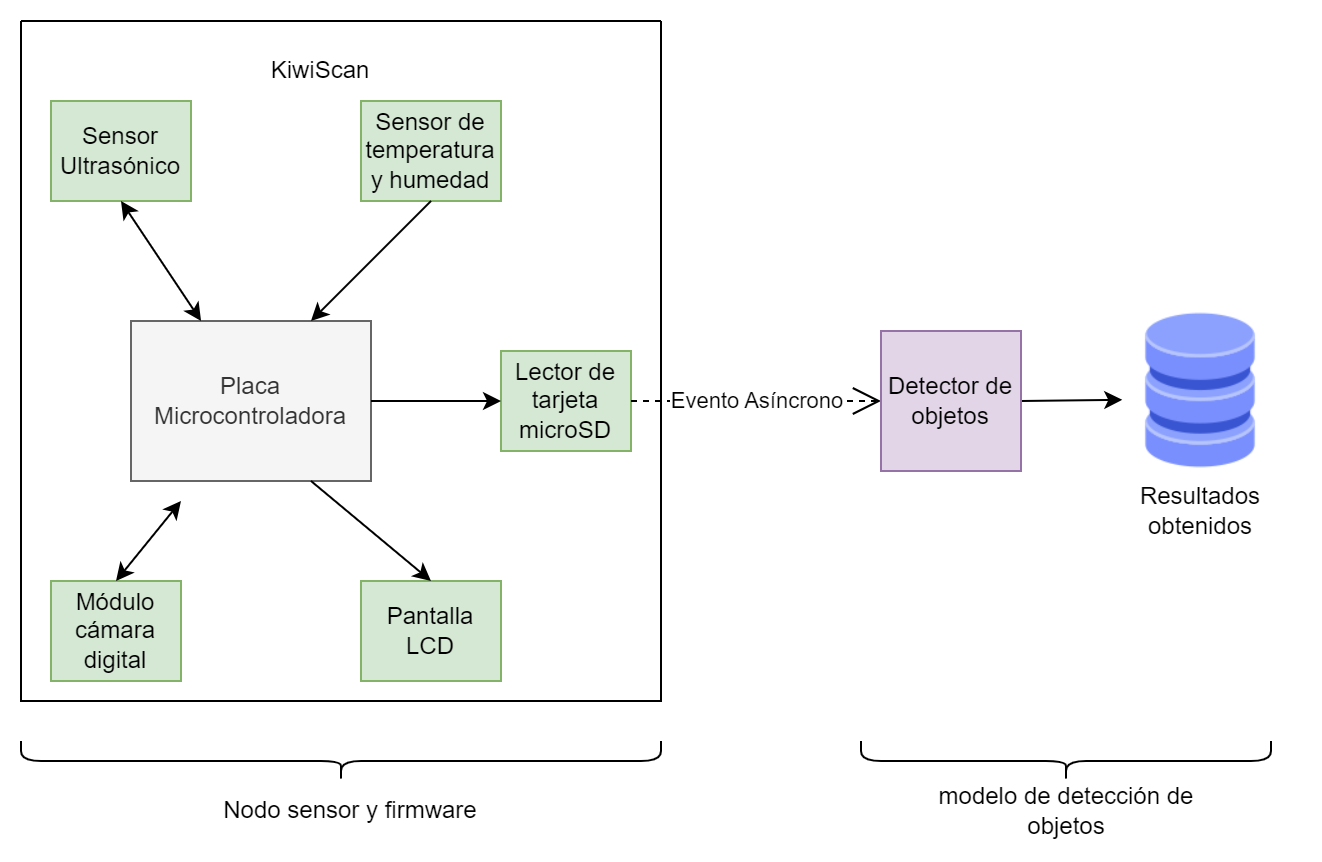
\includegraphics[width=0.9\textwidth, height=0.45\textheight]{./Figures/diagrama_de_componentes.png}
	\caption{Diagrama de componentes.}
	\label{fig:diagrama_de_componentes}
\end{figure}

\vspace{1cm}

El diagrama de componentes ofrece una representación visual clara del sistema KiwiScan y facilita la comprensión de cómo las distintas partes se interconectan y colaboran para cumplir con las tareas de detección de frutos. El flujo de información entre el nodo sensor, el firmware y el modelo de detección de objetos establece una secuencia lógica en la que cada componente desempeña un rol clave para el funcionamiento del sistema.

\subsection{El nodo sensor}

El nodo sensor constituye el elemento físico del sistema, encargado de adquirir imágenes de la plantación de manera automatizada. Este se compone de cámaras y otros sensores que recopilan información relevante, como las condiciones ambientales. Estos dispositivos se conectan al sistema para capturar datos visuales y ambientales que serán procesados posteriormente. Su principal función es proporcionar los datos necesarios para la siguiente fase, asegurando que las imágenes sean de calidad suficiente para permitir la detección de los frutos. A continuación, se describen en detalle los sensores y periféricos seleccionados que forman parte del nodo:

\newpage

\begin{itemize}
\item La cámara Ov7670 es el elemento central para adquirir imágenes en el sistema. Su elección se basó en la capacidad de la cámara para ajustar automáticamente la exposición y el balance de blancos mantiene una calidad de imagen uniforme, incluso bajo condiciones de iluminación cambiantes. Esta característica es especialmente valiosa en las plantaciones de kiwi, donde la disposición de las hojas genera contrastes y sombras, y la iluminación varía según la hora del día, lo que permite optimizar la calidad de las imágenes obtenidas en diferentes entornos de luz.

\item El sensor de temperatura y humedad DHT11 recopila datos ambientales que complementan la información visual y  permiten obtener un perfil más completo de las condiciones en las que se encuentra la plantación. Estas mediciones pueden ajustarse para optimizar los algoritmos de procesamiento de imágenes y así mejorar la detección de frutos en situaciones adversas.
\item El sensor ultrasónico HC-SR04 se utiliza para asegurar que las imágenes capturadas se realicen a una distancia óptima de los frutos, lo que garantiza que los kiwis ocupen un espacio adecuado dentro del campo de visión de la cámara.
\item La pantalla LCD funciona como una interfaz directa para el usuario en el nodo sensor. Presenta información relevante, como la distancia medida por el sensor ultrasónico, los datos de temperatura y humedad proporcionados por el DHT11, y el estado de las imágenes capturadas por la cámara.
\item El lector de tarjetas SD es crucial para el almacenamiento de las imágenes capturadas y los datos ambientales registrados por los sensores.
\item La placa de desarrollo STM32 Nucleo-F429ZI actúa como el cerebro del nodo sensor. Procesa las señales de los sensores y gestiona la adquisición de datos. La STM32 se comunica con los sensores mediante diversos protocolos, como UART para el sensor ultrasónico e I2C para la pantalla LCD, lo que asegura un funcionamiento coordinado del nodo.
\end{itemize}

El nodo sensor no solo recopila datos visuales y ambientales, sino que también ofrece una interfaz directa para los operadores mediante la pantalla LCD y almacena la información adquirida en el recorrido. Estas funciones permiten que el sistema funcione de manera autónoma, registrando datos valiosos para su análisis posterior. Además, la modularidad del nodo facilita la expansión del sistema en futuras versiones, con la posibilidad de incorporar más sensores o mejorar su capacidad de procesamiento. La figura \ref{fig:nodo_sensor} muestra la composición de este nodo.

\vspace{1cm}

\begin{figure}[htbp]
	\centering
	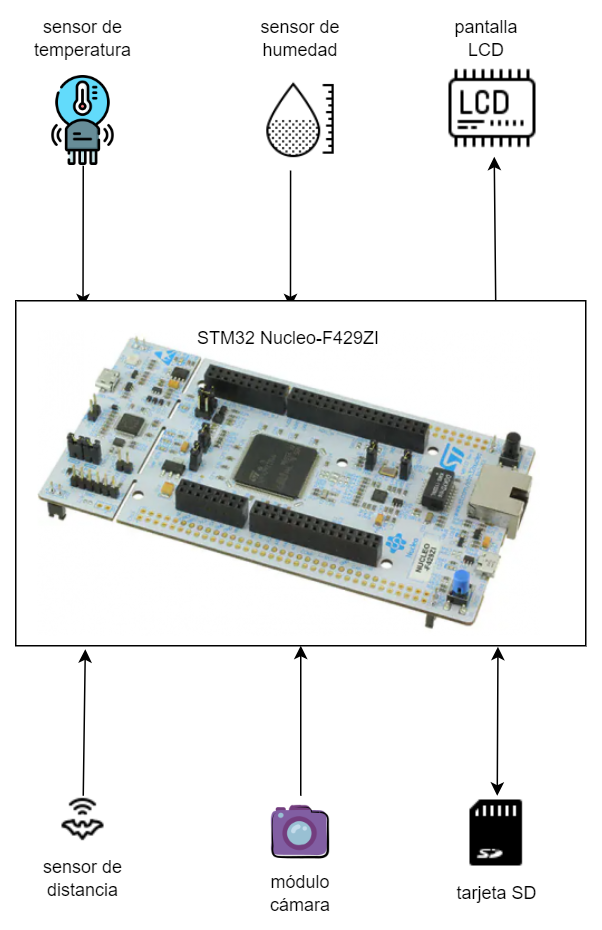
\includegraphics[width=0.6\textwidth, height=0.39\textheight]{./Figures/nodo_sensor.png}
	\caption{Nodo sensor y sus componentes.}
	\label{fig:nodo_sensor}
\end{figure}

\vspace{1cm}

\newpage

\subsection{El firmware del sistema}

El firmware controla la lógica operativa del sistema y actúa como el vínculo entre los sensores, el procesamiento de datos y el almacenamiento de información. Además, coordina las actividades de los diversos componentes del hardware y ejecuta cada tarea de manera precisa para maximizar la eficiencia operativa del sistema. Su diseño se basa en una estructura por capas que optimiza la organización y legibilidad del código, lo que simplifica la gestión y el mantenimiento de su complejidad. La figura \ref{fig:firmware_general} muestra la división en capas del firmware desarrollado.

\newpage

\vspace{1cm}

\begin{figure}[htbp]
	\centering
	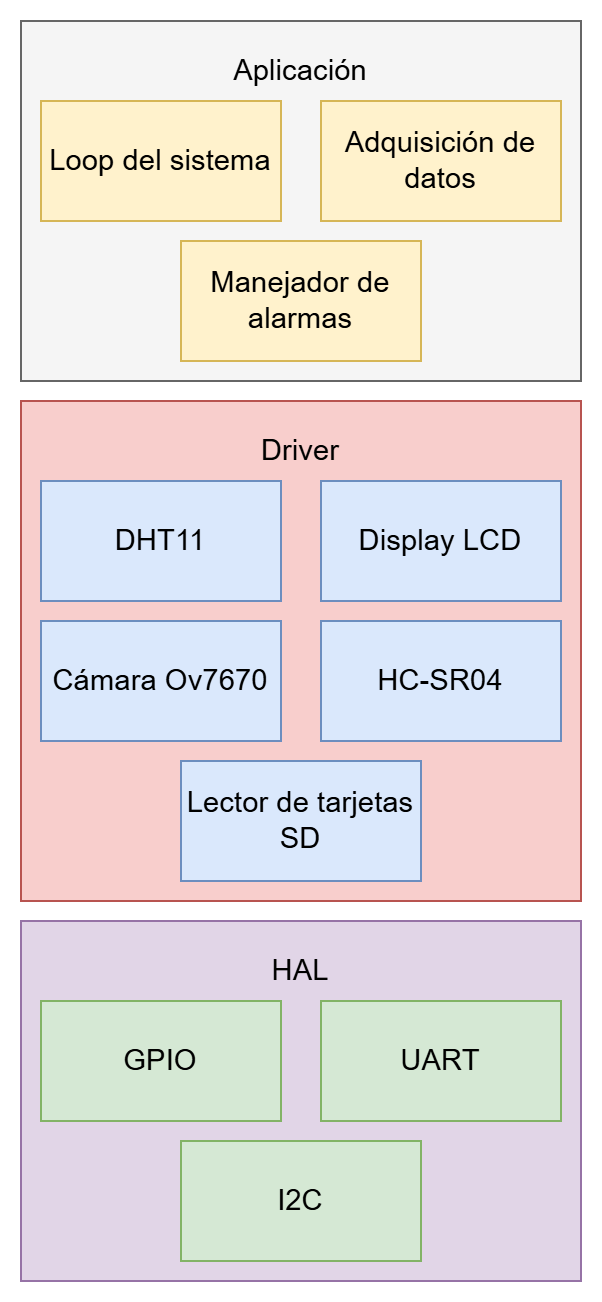
\includegraphics[width=0.5\textwidth, height=0.7\textheight]{./Figures/firmware_general.png}
	\caption{Capas del firmware.}
	\label{fig:firmware_general}
\end{figure}

\vspace{1cm}

\subsubsection{Capa HAL}

La capa HAL (\textit{Hardware Abstraction Layer}), proporcionada por el fabricante del microcontrolador, representa el nivel más bajo del sistema y permite que las capas superiores interactúen con los periféricos del microcontrolador a través de funciones en lenguaje C. Esta capa abstrae las complejidades del hardware y facilita el acceso a las funcionalidades del microcontrolador, lo que mejora la eficiencia y modularidad del sistema. A continuación, se describen los módulos clave de la capa HAL utilizados en el firmware:

\begin{itemize}
\item GPIO (\textit{General Purpose Input/Output}): proporciona funciones para el manejo de las entradas y salidas digitales del microcontrolador. En este sistema, la capa de aplicación utiliza las funciones GPIO para gestionar los indicadores LED de depuración y controlar el encendido y reinicio del sistema. Estos elementos resultan fundamentales para verificar el correcto funcionamiento y estado del nodo sensor en tiempo real.
\item UART (\textit{Universal Asynchronous Receiver-Transmitter}): brinda funciones específicas para la lectura y escritura del puerto UART del microcontrolador, lo que permite la comunicación en serie. El firmware emplea estas funciones UART para establecer un enlace con módulos adicionales, lo que facilita la transmisión de datos sin la necesidad de un reloj compartido. Esta característica es esencial para intercambiar información de manera confiable entre los componentes del sistema.
\item I2C (\textit{Inter-Integrated Circuit}): proporciona funciones para la transmisión y recepción de datos mediante el protocolo I2C, que permite la comunicación con dispositivos externos. En este proyecto, el driver de la pantalla LCD utiliza el protocolo I2C para actualizar la visualización de datos en tiempo real. La implementación del protocolo I2C permite una integración flexible y eficaz de dispositivos adicionales, lo que mejora la interacción entre los distintos módulos del sistema.
\end{itemize}

\subsubsection{Capa drivers}
\label{Capa_drivers}

La capa de drivers, o manejadores de dispositivos, consiste en los controladores desarrollados para facilitar la interacción entre el microcontrolador y el hardware externo. Cada driver se compone de funciones especializadas que permiten el control y gestión de dispositivos específicos. A continuación, se describen los drivers implementados para cada componente del sistema:

Driver de la cámara Ov7670: este controlador permite gestionar la captura de imágenes y configuración de la cámara. Entre sus funciones se incluyen:
\begin{itemize}
\item Iniciar captura de imagen: activa la adquisición de imágenes desde la cámara.
\item Detener captura de imagen: interrumpe el proceso de captura.
\item Pausar captura de imagen: suspende temporalmente la captura de imágenes sin perder la configuración actual.
\item Reanudar captura de imagen: retoma la captura desde el estado pausado.
\item Cambiar la resolución de captura de imagen: ajusta la resolución de imagen para adaptarse a los requisitos del sistema y a las condiciones de operación.
\end{itemize}

Driver para el sensor de temperatura y humedad DHT11: este controlador facilita la adquisición de datos ambientales y ofrece funciones clave para obtener y procesar las lecturas de temperatura y humedad. Las funcionalidades incluidas son:
\begin{itemize}
\item Tomar temperatura: obtiene la temperatura del entorno desde el sensor.
\item Tomar humedad: adquiere el nivel de humedad ambiente.
\item Devolver la temperatura en grados Celsius: convierte y presenta la temperatura en la escala Celsius.
\item Devolver la temperatura en grados Fahrenheit: convierte y muestra la temperatura en la escala Fahrenheit.
\end{itemize}

Driver del sensor ultrasónico HC-SR04: este controlador permite medir la distancia entre el sensor y los objetos cercanos mediante pulsos ultrasónicos. Sus funciones principales son:
\begin{itemize}
\item Enviar señal de eco: emite una señal ultrasónica hacia el objeto.
\item Calcular distancia en centímetros: calcula y devuelve la distancia medida en centímetros.
\item Calcular distancia en metros: calcula y retorna la distancia medida en metros.
\item Detener la señal de eco: interrumpe la emisión de pulsos ultrasónicos.
\end{itemize}

Driver para la pantalla LCD: este controlador gestiona la visualización de datos en la pantalla LCD y ofrece al operador información en tiempo real sobre el estado del sistema. Entre las funciones disponibles se encuentran:
\begin{itemize}
\item Refrescar pantalla: actualiza la información mostrada en la pantalla para reflejar los datos más recientes.
\item Mostrar mensaje en pantalla: presenta un mensaje específico en la pantalla para el usuario.
\item Limpiar pantalla: borra el contenido actual, dejando la pantalla en blanco.
\item Escribir al comienzo de la línea: permite escribir texto desde el inicio de una línea específica.
\item Escribir al final de la línea: escribe texto en la posición final de una línea seleccionada.
\end{itemize}

Driver del lector de tarjetas SD: este controlador permite el almacenamiento seguro y organizado de los datos capturados en una tarjeta SD. Las funciones que incluye son:
\begin{itemize}
\item Escribir en la tarjeta: graba datos en la tarjeta SD para su posterior análisis.
\item Borrar contenido de la tarjeta: elimina los archivos almacenados en la tarjeta.
\item Comprobar espacio en la tarjeta: verifica el espacio libre disponible en la tarjeta SD.
\item Comprobar formateo de la tarjeta: asegura que la tarjeta esté correctamente formateada para evitar errores de lectura/escritura.
\end{itemize}

\newpage

\subsubsection{Capa aplicación}
\label{capa_aplicacion}

La capa de aplicación representa el nivel jerárquico superior del sistema y se implementó sobre el sistema operativo en tiempo real FreeRTOS, lo que permite una mayor escalabilidad del código. Esta capa coordina y organiza la lógica de las funciones avanzadas del sistema mediante tres tareas principales, descritas a continuación:

\begin{itemize}
\item Loop del sistema: esta tarea proporciona la secuencialidad necesaria para que el sistema funcione de manera continua y ordenada. Actúa como el “hilo conductor” de todas las operaciones, gestionando el flujo de actividades y garantizando que cada módulo cumpla su función en el momento oportuno.
\item Adquisición de datos: responsable de leer los datos provenientes de cada sensor, esta tarea asegura que el sistema capture información ambiental y visual de manera constante y precisa. Además, coordina las peticiones de cada sensor para evitar conflictos y optimizar el uso de recursos, permitiendo que la información obtenida esté lista para su posterior procesamiento y análisis.
\item Manejador de alarmas: esta tarea supervisa las condiciones críticas del sistema, activando alarmas ante eventos como desconexión de dispositivos o falta de memoria. El manejador de alarmas proporciona una capa de seguridad adicional, alertando sobre posibles problemas de funcionamiento y evitando fallos en el sistema mediante la implementación de respuestas rápidas y automáticas a estos eventos.
\end{itemize}

\subsection{Modelo de detección de objetos}

El modelo de detección de objetos es el componente encargado de analizar las imágenes adquiridas por el nodo sensor. Este modelo, basado en técnicas de visión por computadora y aprendizaje automático, tiene la capacidad de identificar y contar los frutos presentes en las imágenes, diferenciando entre frutos maduros y aquellos que no lo están. Cabe recordar que, como se mencionó en el capítulo \ref{Aspectos_no_incluidos_en_el_prototipo}, el desarrollo de este modelo no forma parte de este trabajo, pero es un componente esencial en la funcionalidad completa del sistema. 

\newpage

\section{Arquitectura del firmware}

La arquitectura del firmware del sistema está diseñada para optimizar la coordinación y el control de múltiples componentes, asegurando una operación eficiente y una respuesta rápida a eventos internos y externos. Se implementaron dos patrones arquitectónicos principales: el patrón de observar y reaccionar y el de segmentación de procesos, cada uno de ellos cumple funciones específicas dentro de la estructura del firmware.

\subsection{Patrón de observar y reaccionar}

Este patrón mostrado en la figura \ref{fig:patron_de_observar_y_reaccionar} permite que el sistema responda de inmediato a cambios en el entorno o en los estados de los componentes. En la práctica, cada módulo del firmware permanece en constante monitoreo de las señales y datos provenientes de los sensores y dispositivos externos, como el sensor de temperatura y humedad, el sensor ultrasónico y la cámara. Cuando alguno de estos dispositivos genera un cambio relevante en sus lecturas (por ejemplo, una variación de temperatura o una nueva imagen capturada), el sistema ``observa'' esta alteración y automáticamente ``reacciona'' ejecutando las acciones correspondientes, como almacenar los datos en la SD o actualizar la pantalla LCD. Este enfoque facilita una respuesta inmediata a los eventos sin la necesidad de que el sistema esté en modo de consulta continua, esto optimiza el uso de los recursos y reduce la latencia en la toma de decisiones.

\vspace{1cm}
\begin{figure}[htbp]
	\centering
	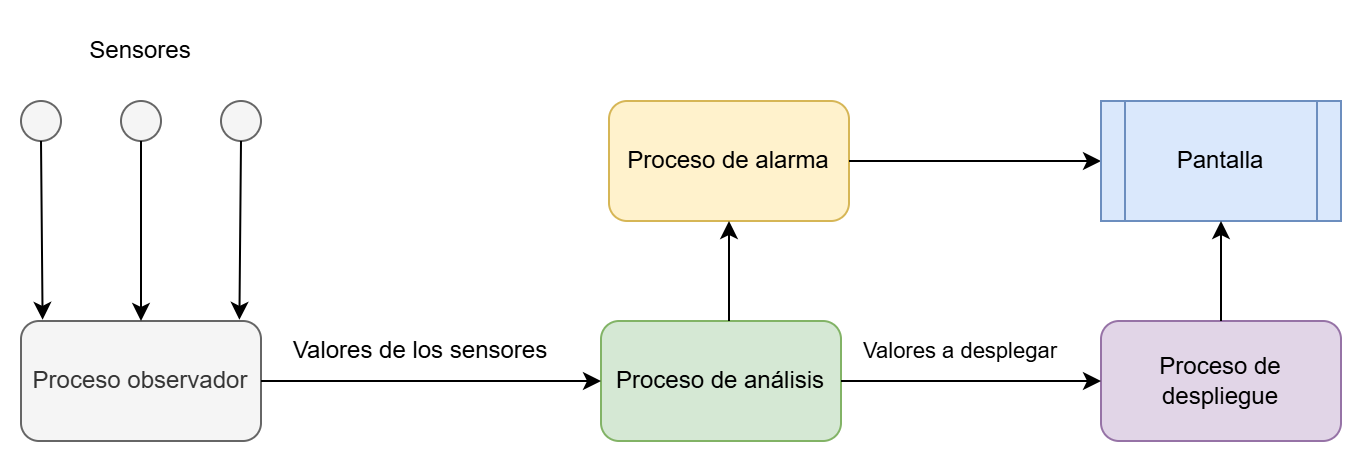
\includegraphics[width=0.9\textwidth, height=0.25\textheight]{./Figures/patron_de_observar_y_reaccionar.png}
	\caption{Patrón de observar y reaccionar.}
	\label{fig:patron_de_observar_y_reaccionar}
\end{figure}
\vspace{1cm}

\newpage

\subsection{Patrón de segmentación de procesos}

Este patrón mostrado en la figura \ref{fig:segmentacion_de_procesos} se utiliza para transformar los datos obtenidos de los sensores, convirtiéndolos de su formato original a una representación adecuada antes de que puedan ser procesados eficazmente. Al realizar esta transformación inicial, el sistema asegura que los datos se presenten de manera uniforme y comprensible, lo que optimiza la precisión y consistencia en las etapas posteriores de procesamiento. Por ejemplo, los valores crudos obtenidos del sensor de temperatura pueden ser transformados en grados Celsius o Fahrenheit según las necesidades del sistema, y los datos del sensor ultrasónico se convierten en metros o centímetros. Esta normalización facilita que otros módulos del firmware interpreten los datos de manera rápida y sin ambigüedades, lo que permite una respuesta más eficiente y coherente en la operación del sistema.

\vspace{1cm}
\begin{figure}[htbp]
	\centering
	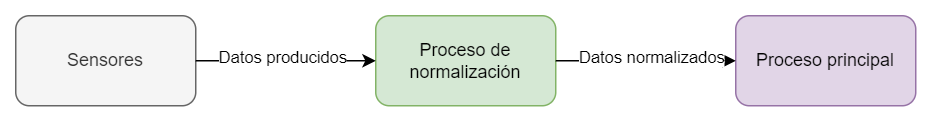
\includegraphics[width=0.9\textwidth, height=0.1\textheight]{./Figures/segmentacion_de_procesos.png}
	\caption{Segmentación de procesos.}
	\label{fig:segmentacion_de_procesos}
\end{figure}
\vspace{1cm}

\section{Módulos del firmware}

Los módulos están organizados en el firmware como funciones independientes que operan de forma coordinada y autónoma. Al segmentar el procesamiento, el firmware asigna tareas específicas a cada módulo, permitiendo que estos funcionen de manera paralela y reduciendo el riesgo de interferencias entre procesos. Así, tareas como la captura de imágenes, el monitoreo ambiental y el manejo de la interfaz de usuario pueden ejecutarse sin interrupciones, manteniendo una operación fluida y eficiente. Además, la segmentación facilita la escalabilidad del firmware, ya que los módulos pueden ser modificados o ampliados sin afectar la arquitectura completa, permitiendo agregar nuevos dispositivos o mejorar funcionalidades en futuras versiones del sistema. Cada módulo mostrado en la figura \ref{fig:modulos_del_firmware} representa a los drivers mencionados en la sección \ref{Capa_drivers}.

\newpage

\vspace{1cm}
\begin{figure}[htbp]
	\centering
	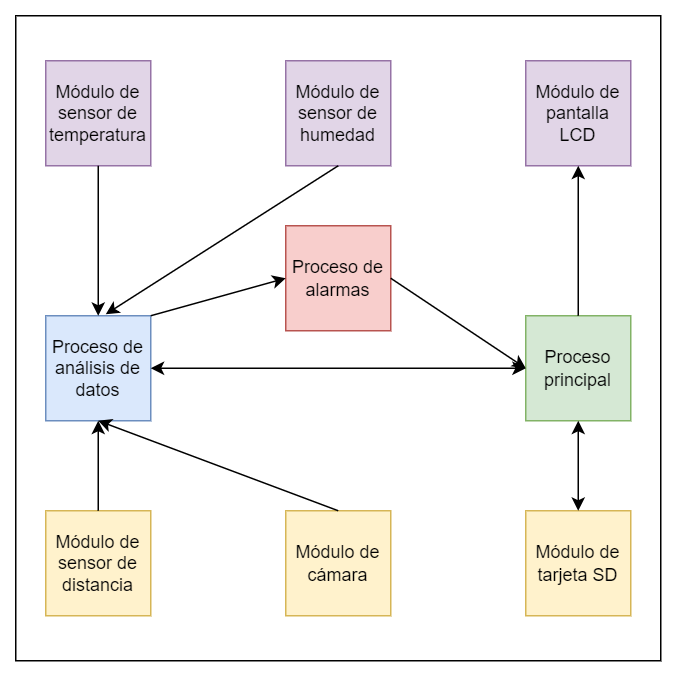
\includegraphics[width=0.9\textwidth, height=0.5\textheight]{./Figures/modulos_del_firmware.png}
	\caption{Módulos del firmware.}
	\label{fig:modulos_del_firmware}
\end{figure}
\vspace{1cm}

Los módulos operan de manera estructurada y siguen una secuencia de pasos específicos para procesar y distribuir la información capturada por el sistema:

\begin{itemize}
\item Módulo de sensor de temperatura: recibe los datos de temperatura directamente del sensor y los transfiere al proceso de análisis de datos para su interpretación y uso en el sistema.
\item Módulo de sensor de humedad: recolecta las lecturas de humedad y las dirige al proceso de análisis de datos, donde estas mediciones contribuyen a la evaluación del entorno del sistema.
\item Monitor de sensor de distancia: captura los datos del sensor de distancia y los envía al proceso de análisis de datos, permitiendo la verificación de la proximidad de los objetos capturados por la cámara.
\item Módulo de pantalla LCD: asegura que la información generada por el sistema, incluidos los datos de sensores y el estado operativo, se muestre correctamente en el display, proporcionando al usuario una visión clara y accesible.

\newpage

\item Módulo de tarjeta SD: gestiona el almacenamiento permanente de datos en la tarjeta SD, al recibir la información ya procesada desde el proceso principal. Cuando el sistema lo requiere, consulta la memoria para recuperar datos históricos y los transfiere de vuelta al proceso principal.
\item Módulo de cámara: realiza las capturas de imagen y las dirige al proceso de análisis de datos, donde se realiza el procesamiento visual o cualquier análisis relevante que se integre a los cálculos generales.
\item Proceso de análisis de datos: procesa los datos obtenidos por los sensores, generando los cálculos necesarios para obtener parámetros clave del entorno. Una vez procesados, envía estos resultados al proceso principal o, si se detecta algún valor fuera de lo normal, lo comunica directamente al proceso de alarmas.
\item Proceso de alarmas: recibe las alertas generadas por el proceso de análisis de datos cuando se detectan valores anómalos. Actúa generando las alarmas correspondientes y las envía al proceso principal para su gestión.
\item Proceso principal: coordina el sistema central, gestionando la solicitud y envío de datos al módulo de almacenamiento en la tarjeta SD y transfiriendo los resultados relevantes al módulo de pantalla LCD, manteniendo una interacción eficiente y fluida entre los componentes.
\end{itemize}

\section{Desarrollo del firmware}

Para el desarrollo del firmware se empleó STM32CubeIDE, el entorno de desarrollo integrado (IDE) oficial proporcionado por STMicroelectronics. Este IDE ofrece un conjunto de herramientas y bibliotecas diseñadas específicamente para facilitar el trabajo con microcontroladores de la serie STM32. 

El firmware se implementó sobre FreeRTOS, un sistema operativo en tiempo real ampliamente utilizado en sistemas embebidos. En este desarrollo se integraron varias de las funcionalidades de FreeRTOS, como las colas para la transferencia ordenada de datos entre tareas, los semáforos para la sincronización entre procesos, y el uso de tareas específicas para segmentar las funciones del firmware. Además, se configuraron diversas interrupciones que permiten al sistema reaccionar instantáneamente ante eventos externos, como la llegada de datos de un sensor o la detección de un cambio en el entorno de trabajo.

Este diseño modular del firmware, permite la implementación de colas y semáforos, el sistema logra una comunicación eficiente entre sus distintos módulos, manteniendo la integridad de los datos y evitando bloqueos o conflictos en el flujo de información.

En la Figura \ref{fig:DdF_firmware} se presenta un diagrama de flujo que describe el proceso de inicialización del firmware. Este diagrama ilustra cada uno de los pasos que el sistema sigue desde el inicio, pasando por la configuración de los periféricos y la inicialización de las tareas del sistema, hasta el punto en que el firmware queda listo para operar. La organización detallada del flujo de inicialización asegura que cada módulo y sensor del nodo funcione correctamente y en el orden adecuado, garantizando la estabilidad y eficiencia del sistema durante su funcionamiento.

\vspace{1cm}
\begin{figure}[htbp]
	\centering
	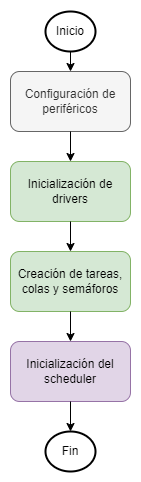
\includegraphics[width=0.3\textwidth, height=0.6\textheight]{./Figures/DdF_firmware.png}
	\caption{Diagrama de flujo de inicialización del firmware.}
	\label{fig:DdF_firmware}
\end{figure}
\vspace{1cm}

Para el control del sistema se crearon dos tareas sobre freeRTOS, que se comunican
y se sincronizan a través de colas y semáforos.

\newpage

\subsection{Tarea adquisición de datos}

La tarea de adquisición de datos cumple un rol esencial en la obtención de las lecturas de los sensores y en la garantía de un flujo continuo y preciso de información hacia el sistema. Esta tarea sigue un flujo estructurado, mostrado en el diagrama de flujo de la Figura \ref{fig:DdF_tarea_adquisición_datos}, donde cada paso asegura que los datos sean recogidos y procesados de manera eficiente.

El proceso de adquisición comienza verificando la cola de adquisición para detectar si existen solicitudes pendientes de datos. Si la cola contiene datos, la tarea procede a iniciar la lectura de todos los sensores del sistema. Estos datos, una vez adquiridos, se colocan en la cola de datos y alarmas, lo que permite que otros procesos, como el análisis y las alarmas, acceder a la información en tiempo real.

En caso de que la cola de adquisición esté vacía, la tarea de adquisición de datos se bloquea temporalmente para optimizar el uso de recursos, permaneciendo en espera hasta que una nueva solicitud de datos sea recibida en la cola. Esta capacidad de bloqueo y activación automática asegura que el sistema mantenga su eficiencia y libere recursos cuando no se requiera una lectura inmediata, además de garantizar que los datos recogidos sean siempre actuales.

Cada vez que los valores leídos presentan variaciones significativas o caen fuera de los rangos normales, el sistema de alarmas puede actuar en función de estos datos y enviar una alerta al proceso de alarmas, que luego gestiona la respuesta adecuada en el sistema.

\vspace{1cm}
\begin{figure}[htbp]
	\centering
	\includegraphics[width=0.45\textwidth, height=0.45\textheight]{./Figures/DdF_tarea_adquisición_datos.png}
	\caption{Diagrama de flujo tarea de adquisición de datos.}
	\label{fig:DdF_tarea_adquisición_datos}
\end{figure}
\vspace{1cm}

\subsection{Tarea manejador de alarmas}

La tarea de manejador de alarmas supervisa los valores de los sensores para asegurar que se mantengan dentro de los límites permitidos de cada variable. En caso de detectar algún valor fuera de los parámetros establecidos, la tarea activa una alarma para alertar al sistema. El diagrama de flujo de esta tarea puede observarse en la Figura \ref{fig:DdF_tarea_manejador_alarmas}.

Al comenzar el bucle infinito de monitoreo, la tarea inspecciona de manera constante la cola de alarmas en busca de eventos. Si se encuentran datos en esta cola, la tarea analiza la información recibida, que puede indicar dos tipos de eventos: monitorear y enviar.

\begin{itemize}
\item Evento monitorear: la tarea verifica si el valor de cada sensor cae por debajo o excede los valores de límite previamente definidos para cada variable. Si alguno de estos valores infringe los límites, la tarea incrementa una variable que registra la cantidad de alarmas activas en el sistema. Esta información resulta fundamental para monitorear el estado del sistema en tiempo real y detectar situaciones de riesgo de manera inmediata.
\item Evento enviar: se verifica si existen alarmas activas en el sistema. En caso afirmativo, notifica al proceso principal para que ejecute las acciones necesarias, como activar una alerta visual. Esta comunicación garantiza una respuesta rápida y adecuada ante cualquier situación crítica detectada.
\end{itemize}

Cuando no se encuentran datos en la cola de alarmas, la tarea entra en un estado de bloqueo, optimizando el uso de recursos del sistema al detener temporalmente su ejecución hasta que se reciba un nuevo dato en la cola. Esta estructura permite que el sistema opere de manera eficiente, reaccionando ante anomalías únicamente cuando estas ocurren y sin consumir recursos innecesarios en condiciones normales.

\newpage

\vspace{1cm}
\begin{figure}[htbp]
	\centering
	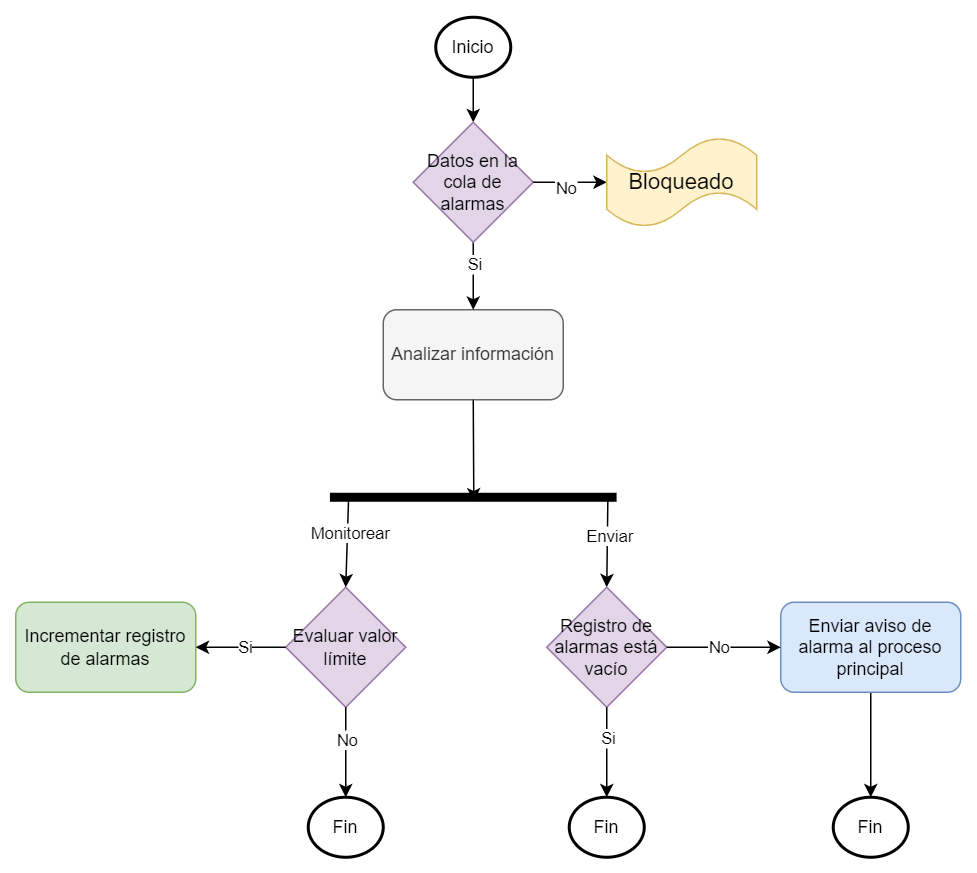
\includegraphics[width=1.0\textwidth, height=0.7\textheight]{./Figures/DdF_tarea_manejador_alarmas.png}
	\caption{Diagrama de flujo de la tarea manejadora de alarmas.}
	\label{fig:DdF_tarea_manejador_alarmas}
\end{figure}
\vspace{1cm}

\newpage
